\documentclass{cshwk}

\title{Wireshark Lab \#2, HTTP}

\begin{document}

\maketitle

\section*{Problem 1. The Basic HTTP GET/response interaction}

\subsection*{Question 1:}

\begin{quote}
    \textbf{Is your browser running HTTP version 1.0 or 1.1? What version of HTTP is the server running?}
\end{quote}

\subsection*{Solutions:}

The http version of my browser can be found in the HTTP GET request. The version of the server can be found in the HTTP OK reply. The details are shown in the Fig.~\ref{fig:http-version-browser} and Fig.~\ref{fig:http-version-server}. \textbf{It shows that the browser is running HTTP version 1.1, and the server is running HTTP version 1.1.}

\begin{figure}[htbp]
    \centering
    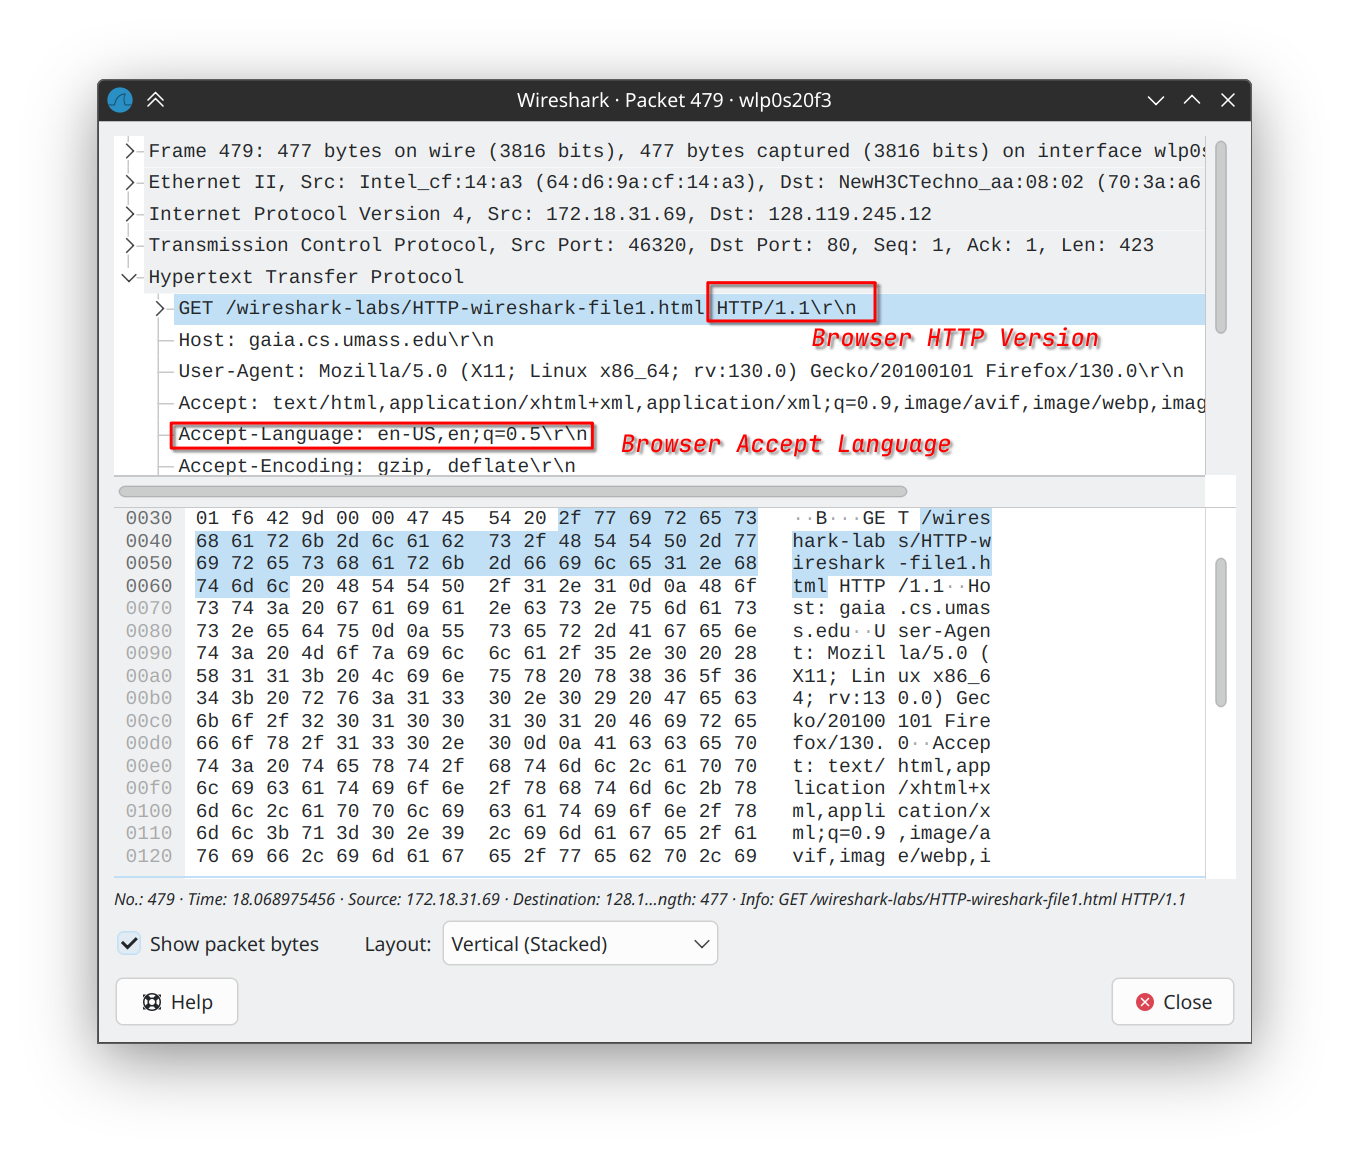
\includegraphics[width=0.6\textwidth]{lab2-1.png}
    \caption{The HTTP version of the browser}
    \label{fig:http-version-browser}
\end{figure}

\begin{figure}[htbp]
    \centering
    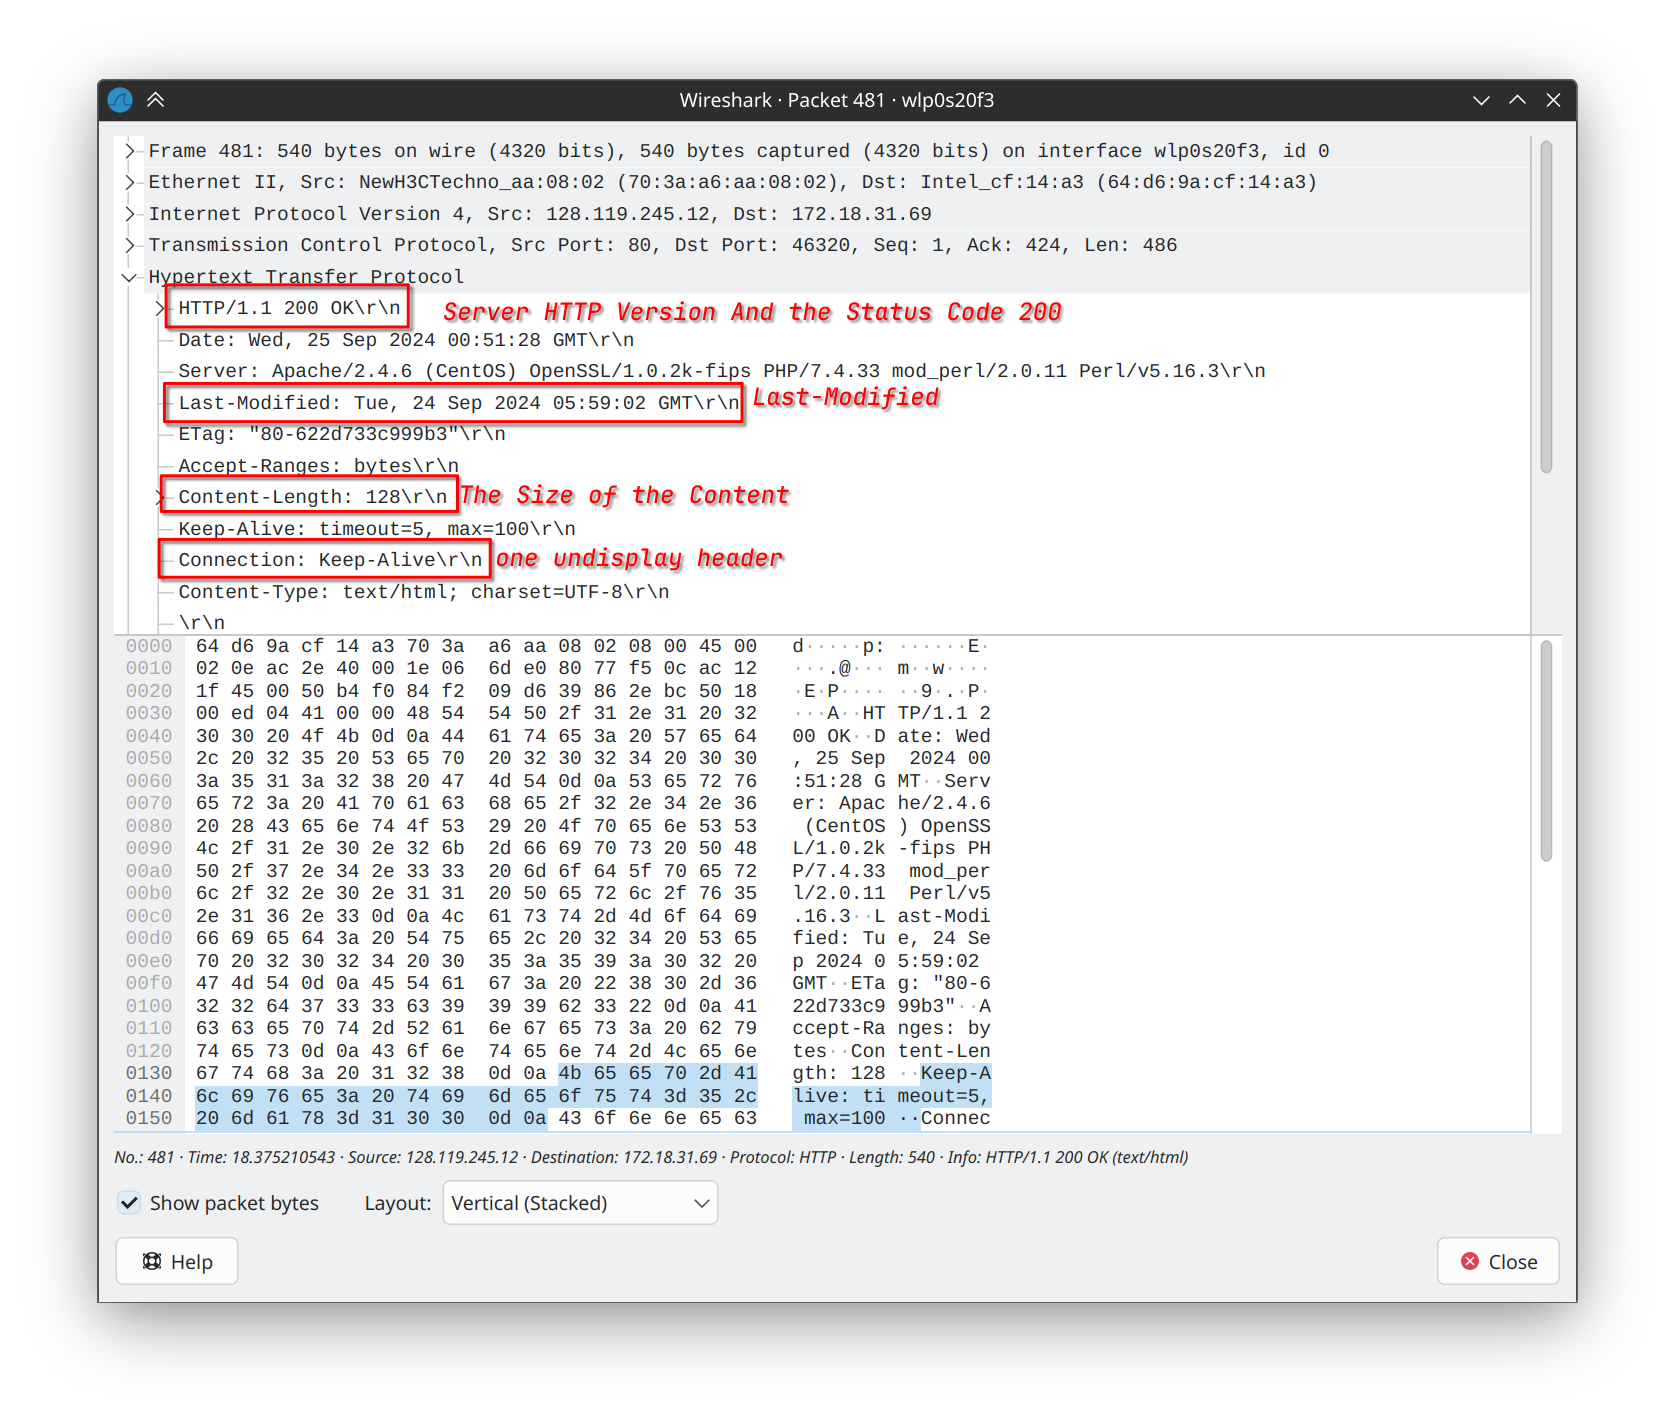
\includegraphics[width=0.6\textwidth]{lab2-2.png}
    \caption{The HTTP version of the server}
    \label{fig:http-version-server}
\end{figure}

\subsection*{Question 2:}

\begin{quote}
    \textbf{What language (if any) does your browser indicate that it can accept to the server?}
\end{quote}

Also, inspect the \texttt{GET} request, and the \texttt{Accept-Language} field in \texttt{HTTP Headers} is shown in Fig.~\ref{fig:http-version-browser}. \textbf{The browser indicates that it can accept \texttt{en-US, en} language to the server.}


\subsection*{Question 3:}

\begin{quote}
    \textbf{What is the IP address of your computer? Of the \href{http://gaia.cs.umass.edu}{gaia.cs.umass.edu} server?}
\end{quote}

\begin{figure}[htbp]
    \centering
    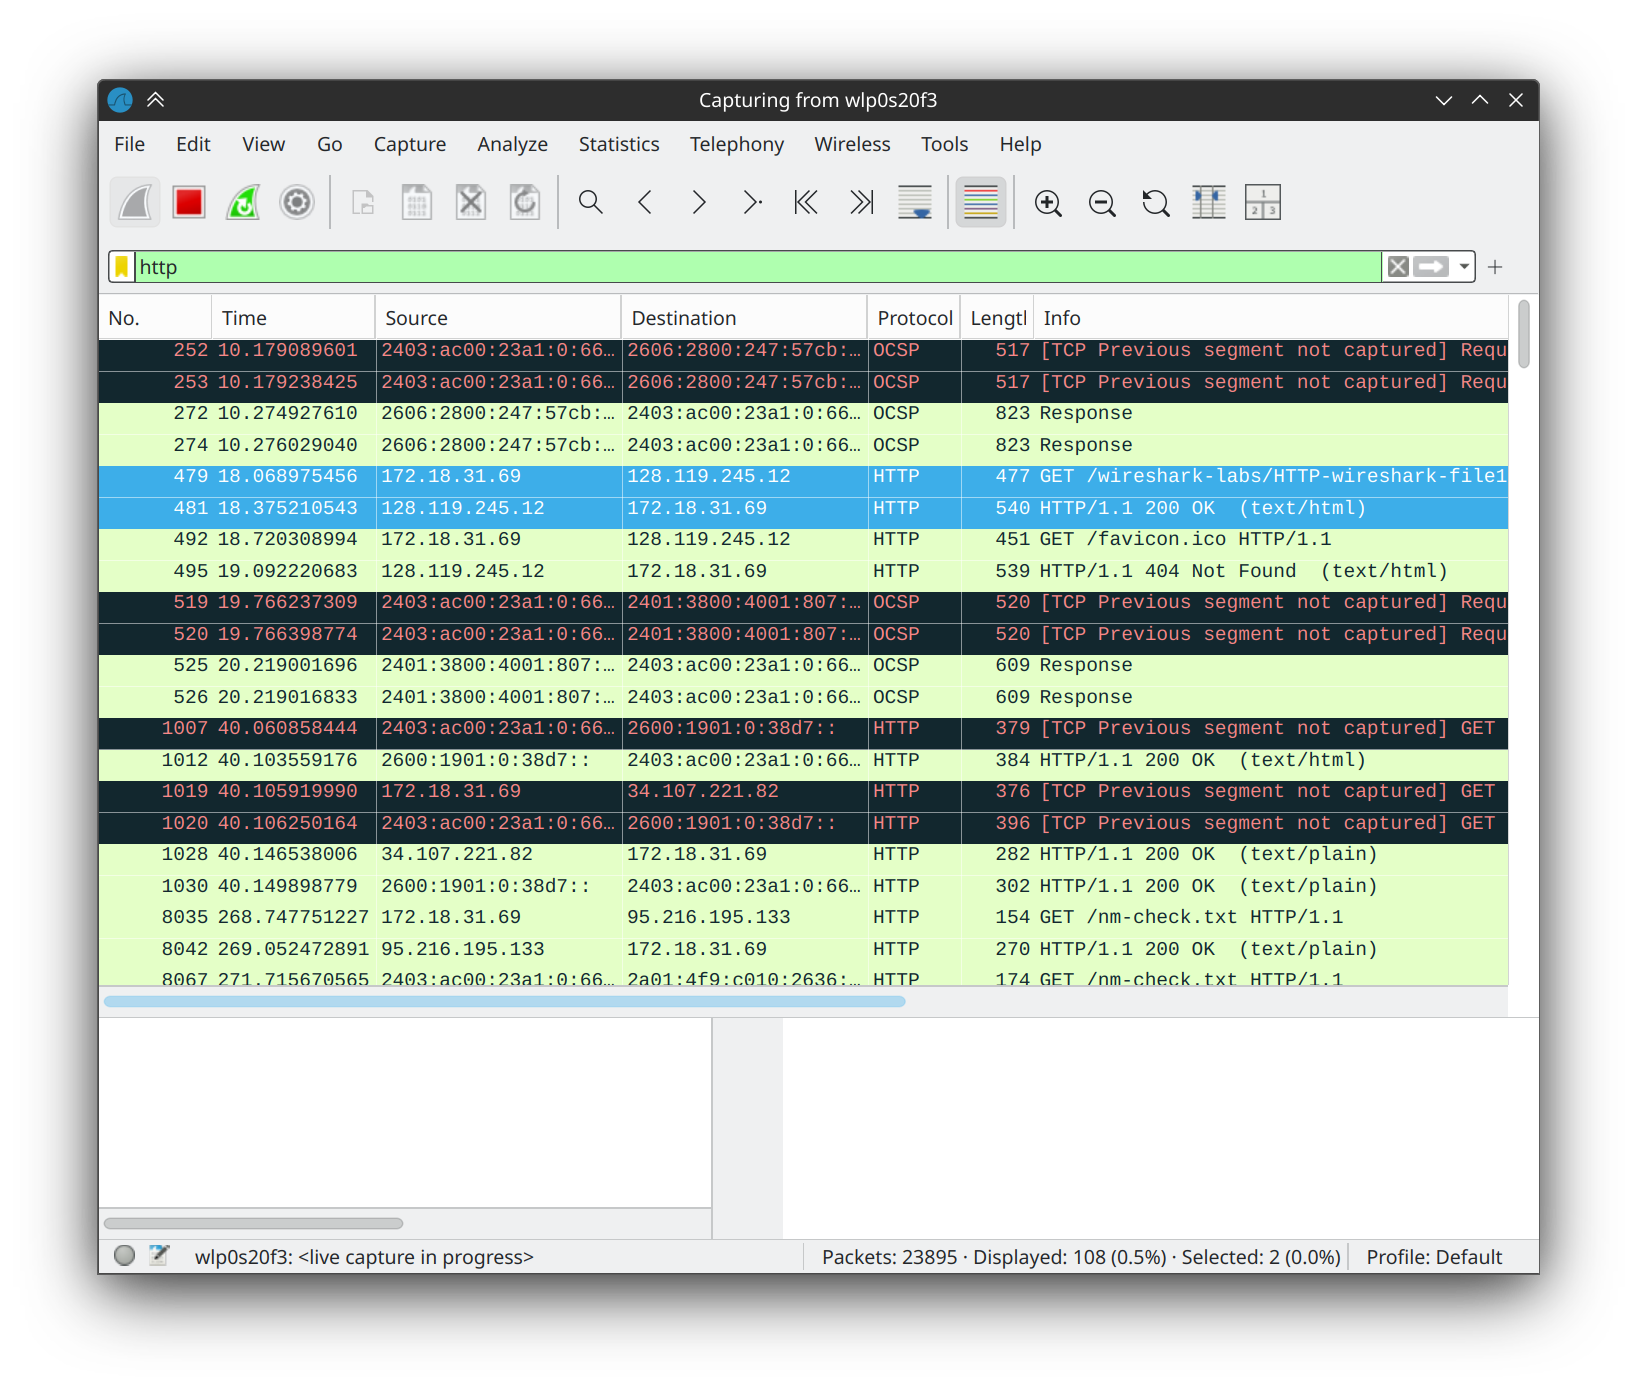
\includegraphics[width=0.6\textwidth]{lab2-3.png}
    \caption{The IP address of the computer and the server}
    \label{fig:ip-address}
\end{figure}

Inspect the \texttt{GET} request, and looking for the \texttt{source} and the \texttt{destination} IP address. The details are shown in the Fig.~\ref{fig:ip-address}. \textbf{The IP address of my computer is \texttt{172.18.31.69} and the IP address of the server is \texttt{128.119.245.12}.}

\subsection*{Question 4:}

\begin{quote}
    \textbf{What is the status code returned from the server to your browser?}
\end{quote}

Inspect the \texttt{HTTP OK} reply, and the \texttt{Status Code} field in \texttt{HTTP} is shown in Fig.~\ref{fig:http-version-server}. \textbf{The status code returned from the server to the browser is \texttt{200 OK}.}

\subsection*{Question 5:}

\begin{quote}
    \textbf{When was the HTML file that you are retrieving last modified at the server?}
\end{quote}

Inspect the \texttt{HTTP OK} reply, and the \texttt{Last-Modified} field in \texttt{HTTP} is shown in Fig.~\ref{fig:http-version-server}. \textbf{The HTML file was last modified on the server on \texttt{Tue, 24 Sep 2024 05:59:02 GMT}.}


\subsection*{Question 6:}
\begin{quote}
    \textbf{How many bytes of content are being returned to your browser?}
\end{quote}

Inspect the \texttt{HTTP OK} reply, and the \texttt{Content-Length} field in \texttt{HTTP} is shown in Fig.~\ref{fig:http-version-server}. \textbf{The number of bytes of content being returned to the browser is \texttt{128}.}

\subsection*{Question 7:}
\begin{quote}
    \textbf{By inspecting the raw data in the packet content window, do you see any headers within the data that are not displayed in the packet-listing window?}
\end{quote}

Inspect the \texttt{HTTP OK} reply, and the \texttt{Raw} field in \texttt{HTTP} is shown in Fig.~\ref{fig:http-version-server}. \textbf{Yes, there are headers within the data that are not displayed in the packet-listing window. For example: \texttt{Content-Type: text/html; charset=UTF-8}, \texttt{Connection: keep-alive}, etc.}



\section*{Problem 2. The HTTP CONDITIONAL GET/response}

Follow the instructions, open the target URL in the browser, and inspect the \texttt{HTTP GET} request and the \texttt{HTTP OK} reply. The results are shown in Fig.~\ref{fig:http-conditional-get}.


\begin{figure}[htbp]
    \centering
    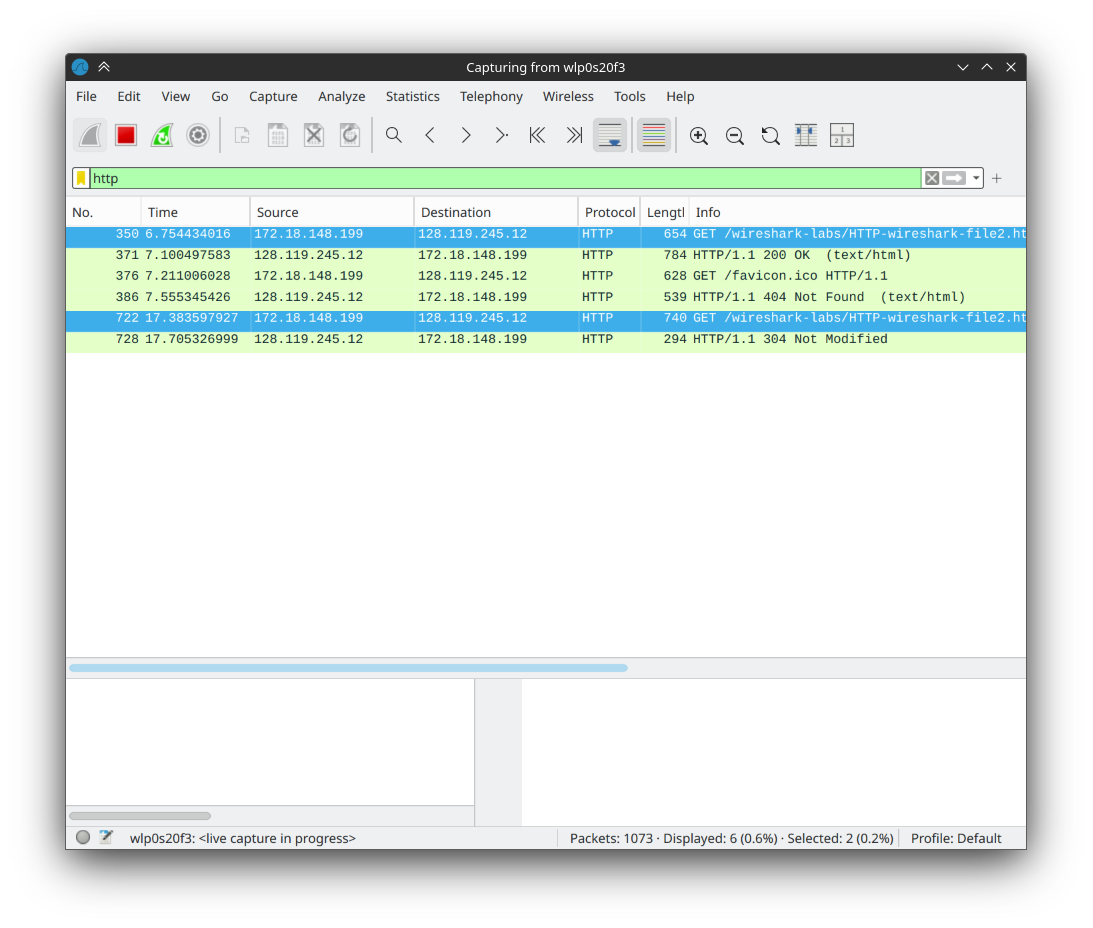
\includegraphics[width=0.6\textwidth]{lab2-4.png}
    \caption{The HTTP CONDITIONAL GET/response}
    \label{fig:http-conditional-get}
\end{figure}

\subsection*{Question 8:}
\begin{quote}
    \textbf{Inspect the contents of the first HTTP GET request from your browser to the server. Do you see an “IF-MODIFIED-SINCE” line in the HTTP GET?}
\end{quote}

The details of the first \texttt{HTTP GET} request are shown in Fig.~\ref{fig:http-conditional-get-1}. \textbf{No, there is no \texttt{IF-MODIFIED-SINCE} line in the HTTP GET.}


\begin{figure}[htbp]
    \centering
    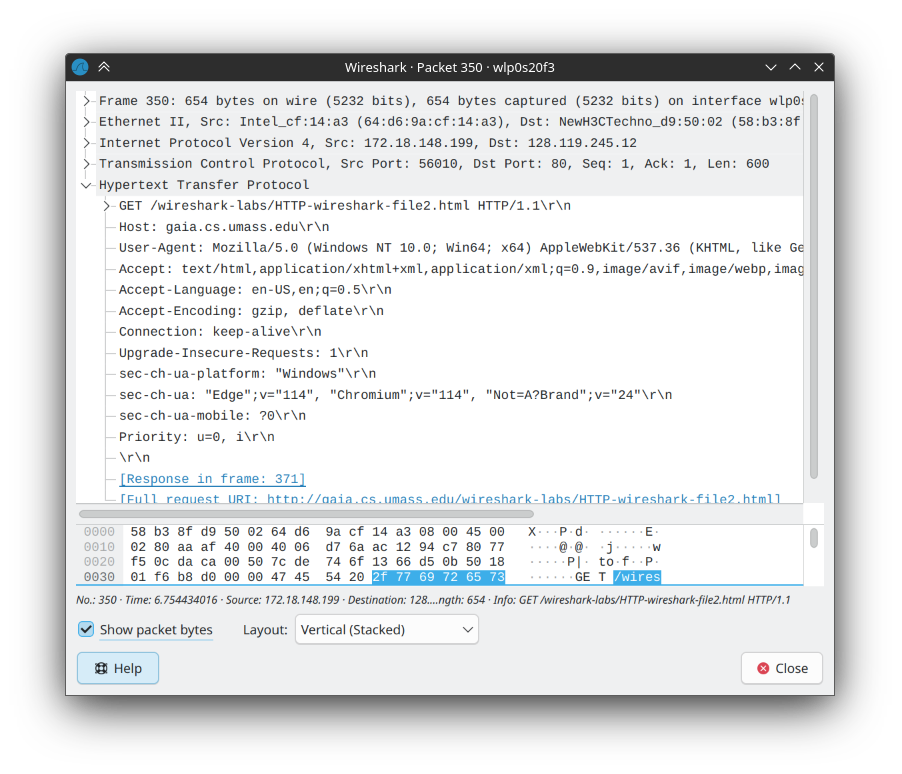
\includegraphics[width=0.6\textwidth]{lab2-5.png}
    \caption{The first HTTP GET request}
    \label{fig:http-conditional-get-1}
\end{figure}

\subsection*{Question 9:}
\begin{quote}
    \textbf{Inspect the contents of the server response. Did the server explicitly return the contents of the file?}
\end{quote}

The details of the server response are shown in Fig.~\ref{fig:http-conditional-get-1-response}. From the \texttt{text-based response message}, we can see that the server explicitly returns the contents of the file. \textbf{Therefore, yes, the server explicitly returns the contents of the file.}


\begin{figure}[htbp]
    \centering
    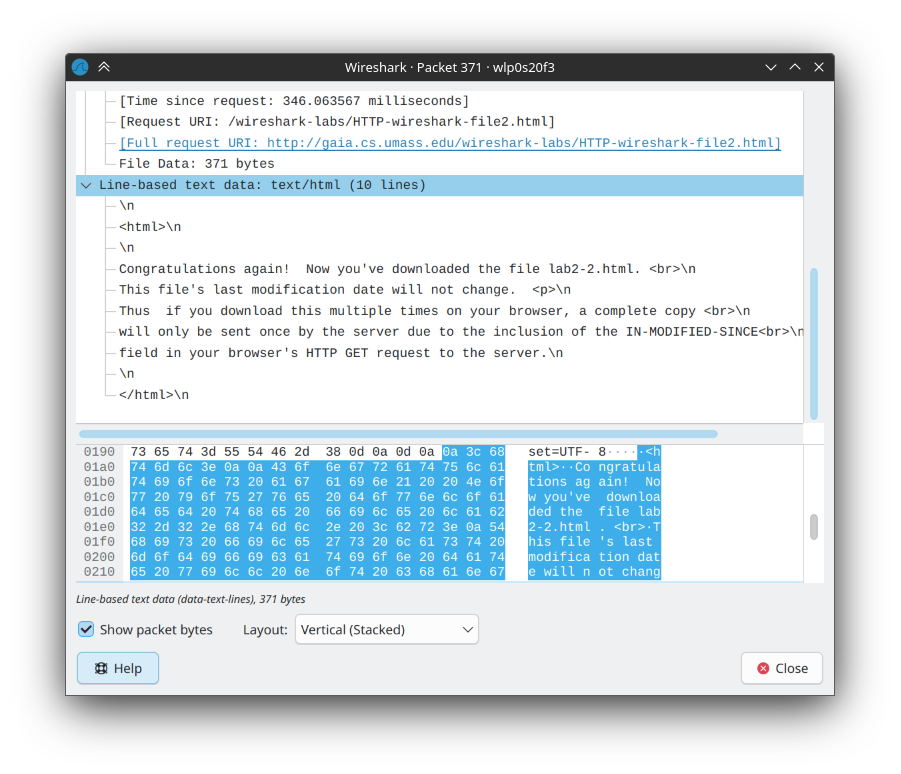
\includegraphics[width=0.6\textwidth]{lab2-6.png}
    \caption{The first HTTP GET response}
    \label{fig:http-conditional-get-1-response}
\end{figure}

\subsection*{Question 10:}
\begin{quote}
    \textbf{Now inspect the contents of the second HTTP GET request from your browser to the server. Do you see an “IF-MODIFIED-SINCE:” line in the HTTP GET? If so, what information follows the “IF-MODIFIED-SINCE:” header?}
\end{quote}

The details of the second \texttt{HTTP GET} request are shown in Fig.~\ref{fig:http-conditional-get-2}. The \texttt{IF-MODIFIED-SINCE} line is visible in the selected field. \textbf{There is an \texttt{IF-MODIFIED-SINCE} line in the HTTP GET request. The information following the \texttt{IF-MODIFIED-SINCE} header is \texttt{Sat, 28 Sep 2024 05:59:02 GMT},} which is the time the file was last modified, as indicated in the first response.


\begin{figure}[htbp]
    \centering
    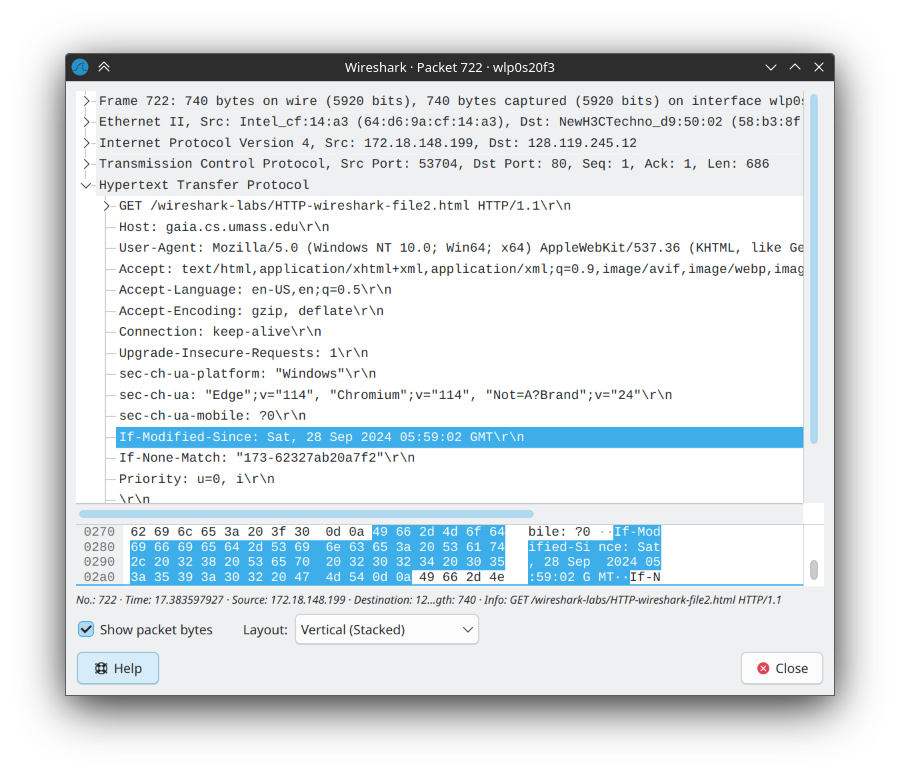
\includegraphics[width=0.6\textwidth]{lab2-7.png}
    \caption{The second HTTP GET request}
    \label{fig:http-conditional-get-2}
\end{figure}

\subsection*{Question 11:}
\begin{quote}
    \textbf{What is the HTTP status code and phrase returned from the server in response to this second HTTP GET? Did the server explicitly return the contents of the file? Explain.}
\end{quote}

The details of the second server response are shown in Fig.~\ref{fig:http-conditional-get-2-response}. From the selected field, we can see that the server returns the status code \texttt{304 Not Modified}. \textbf{The server did not explicitly return the file's contents.} This status code indicates that the file has not been modified since it was last retrieved by the browser, so the server does not resend the file's contents. \textbf{This is the purpose of a conditional GET, which leverages the browser's cache to reduce network traffic.}



\begin{figure}[htbp]
    \centering
    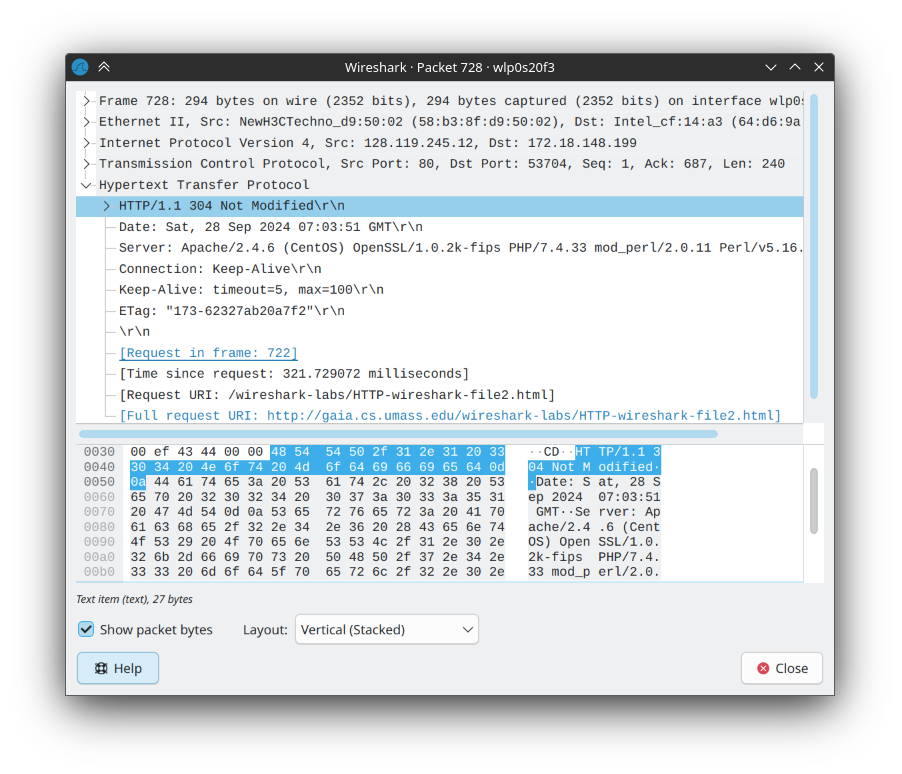
\includegraphics[width=0.6\textwidth]{lab2-8.png}
    \caption{The second HTTP GET response}
    \label{fig:http-conditional-get-2-response}
\end{figure}

\section*{Problem 3. Retrieving Long Documents}

Following the instructions, open the target URL in the browser, and inspect the \texttt{HTTP GET} request and the \texttt{HTTP OK} reply. The results are shown in Fig.~\ref{fig:http-long-documents}.

\begin{figure}[htbp]
    \centering
    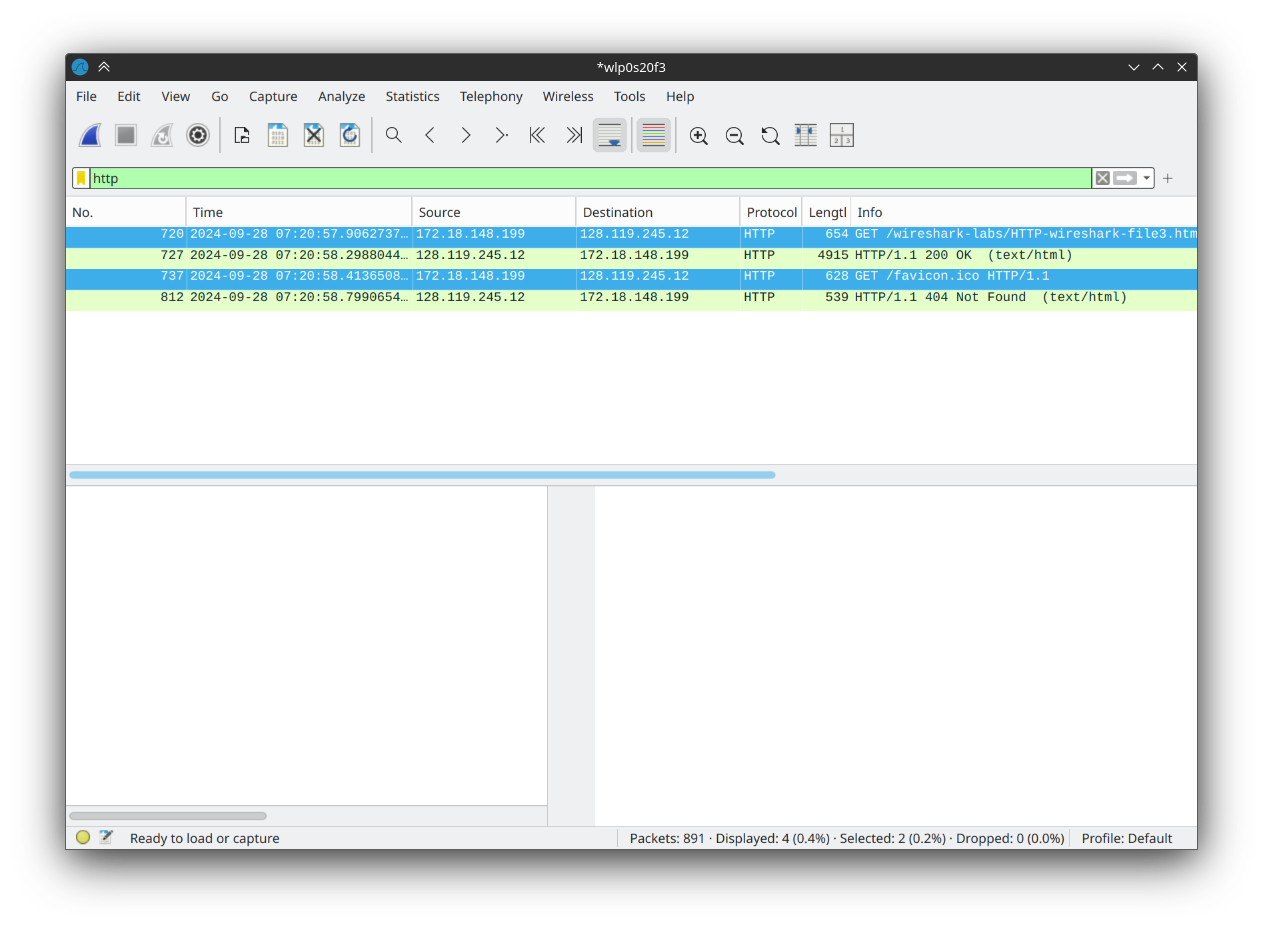
\includegraphics[width=0.6\textwidth]{lab2-9.png}
    \caption{The HTTP GET/response for long documents}
    \label{fig:http-long-documents}
\end{figure}

\subsection*{Question 12:}
\begin{quote}
    \textbf{How many HTTP GET request messages did your browser send? Which packet number in the trace contains the GET message for the Bill or Rights?}
\end{quote}

Inspect the \texttt{HTTP GET} request, as shown in Fig.~\ref{fig:http-long-documents}. There are 2 \texttt{HTTP GET} request messages. The packet number in the trace that contains the GET message for the Bill of Rights is the first \texttt{HTTP GET} request, which is packet No.~720.

\subsection*{Question 13:}
\begin{quote}
    \textbf{Which packet number in the trace contains the status code and phrase associated with the response to the HTTP GET request?}
\end{quote}

Inspect the corresponding `HTTP OK` reply for packet No.~720, as shown in Fig.~\ref{fig:http-long-documents}. It indicates a response code of \texttt{200 OK}. The packet number in the trace that contains the status code and phrase associated with the response to the HTTP GET request is packet No.~727.

\subsection*{Question 14:}
\begin{quote}
    \textbf{What is the status code and phrase in the response?}
\end{quote}
Inspect the \texttt{HTTP OK} reply, focusing on the \texttt{Status Code} field in \texttt{HTTP}, as shown in Fig.~\ref{fig:http-long-documents-response}. The status code and phrase in the response is \texttt{200 OK}, which is highlighted as the selected field.
\begin{figure}[htbp]
    \centering
    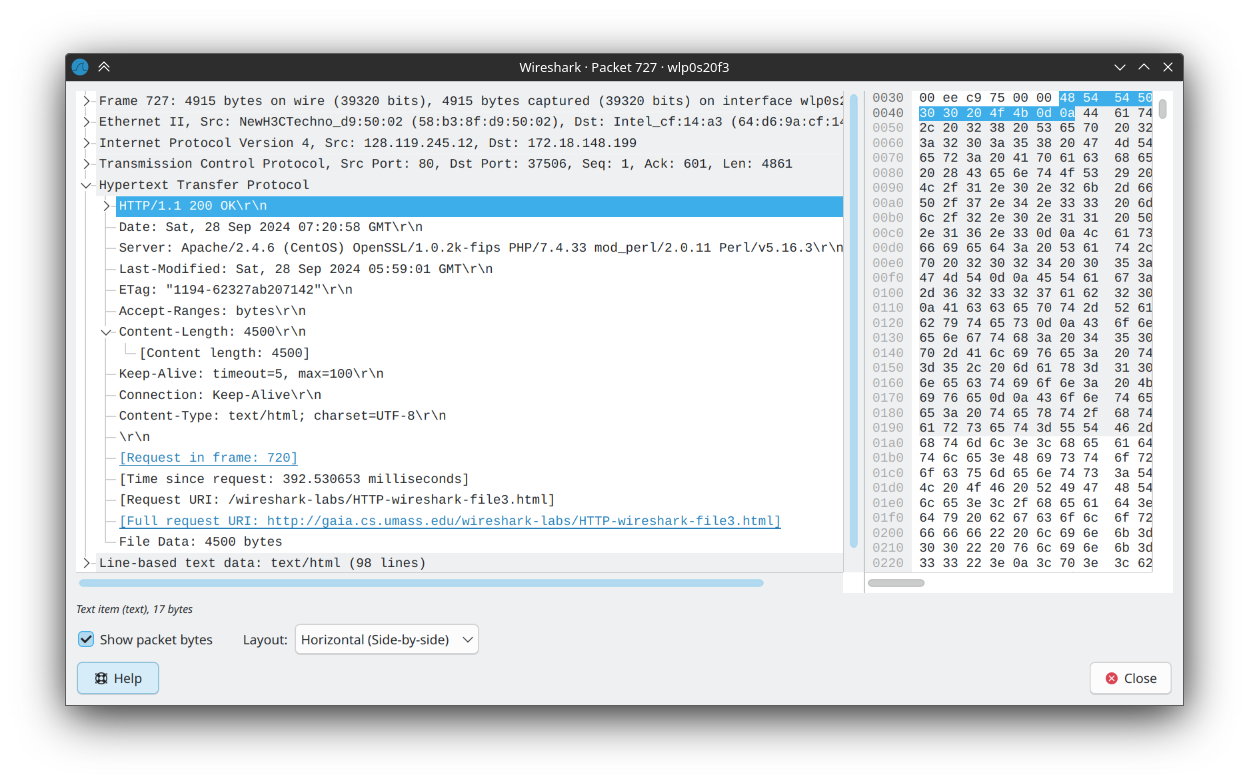
\includegraphics[width=0.6\textwidth]{lab2-10.png}
    \caption{The HTTP OK reply for long documents}
    \label{fig:http-long-documents-response}
\end{figure}

\subsection*{Question 15:}
\begin{quote}
    \textbf{How many data-containing TCP segments were needed to carry the single HTTP response and the text of the Bill of Rights?}
\end{quote}

Inspect the \texttt{HTTP OK} response, and observe the \texttt{TCP} field in \texttt{HTTP} as shown in Fig.~\ref{fig:http-long-documents-response-tcp}. Only one TCP segment contains data, sufficient to carry both the single HTTP response and the text of the Bill of Rights, with a packet length of \texttt{4861 bytes}.

\begin{figure}[htbp]
    \centering
    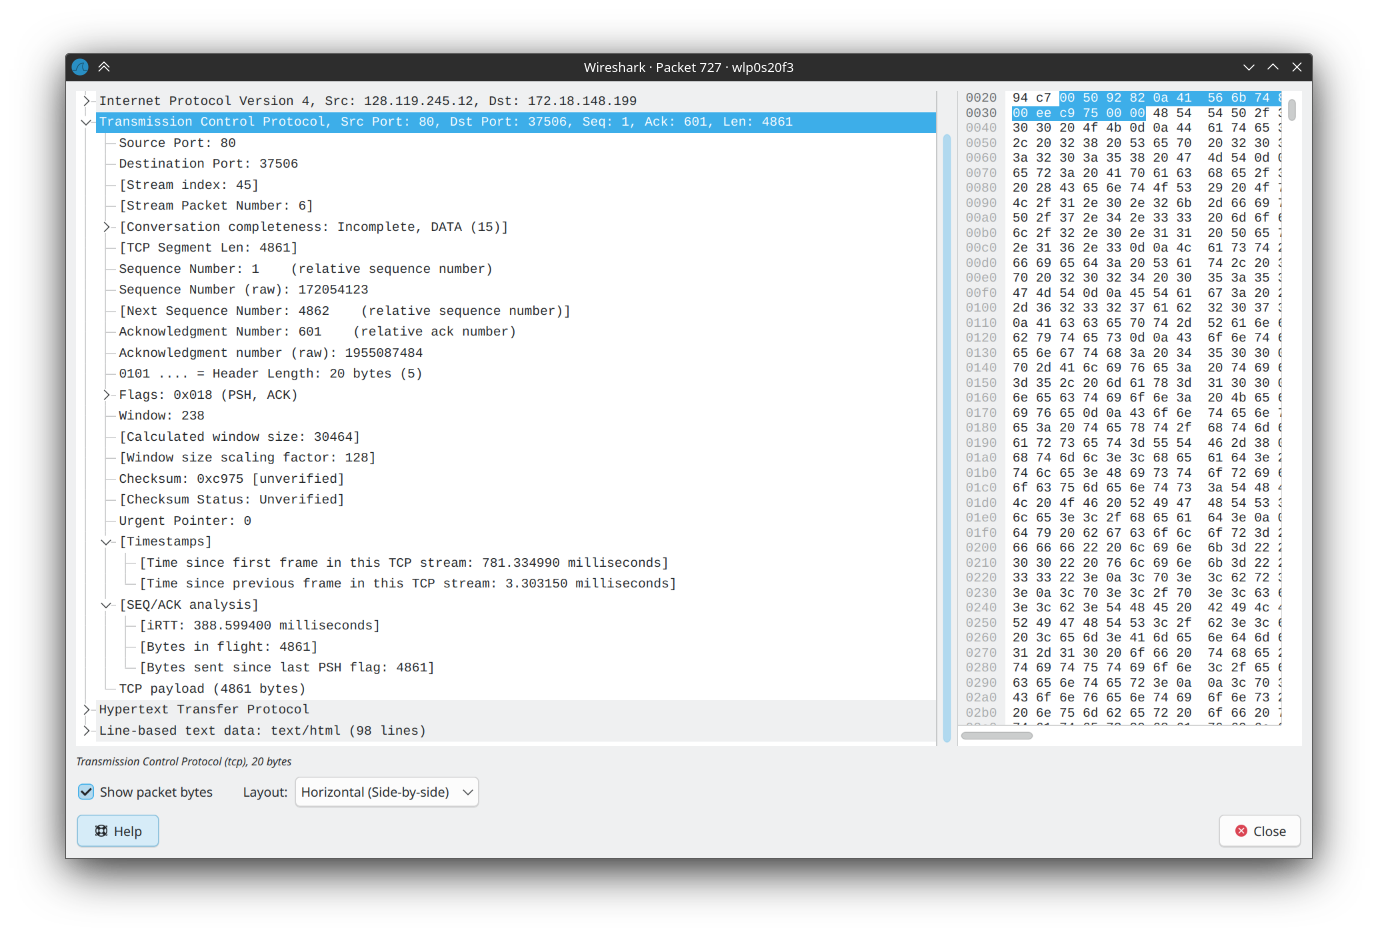
\includegraphics[width=0.9\textwidth]{lab2-11.png}
    \caption{The TCP segment for long documents}
    \label{fig:http-long-documents-response-tcp}
\end{figure}

\end{document}